\documentclass[12pt]{article}

\usepackage{scicite,times,graphicx,float,hyperref}
\usepackage[skip=0pt]{caption}
\usepackage[utf8]{inputenc}
\usepackage{enumitem}
\usepackage{booktabs}
\usepackage{siunitx}

%%%%%%%%%%%%%%%%%%%%%%%%%%%%%%%%%%%%%%%%%%%%%%%%%%%%%%%%%%%%%%%%%%%%%%%%%%% PREAMBLE %%%%%%%%%%%%%%%%%%%%%%%%%%%%%%%%%%%%%%%%%%%%%%%%%%%%%%%%%%%%%%%%%%%%%%%%%%%

\topmargin -1.0cm
\oddsidemargin 0.0cm 
\textwidth 16cm 
\textheight 23cm
\footskip 1.0cm

\newenvironment{sciabstract}{%
\begin{quote} \bf}
{\end{quote}}

\newcounter{lastnote}
\newenvironment{scilastnote}{%
  \setcounter{lastnote}{\value{enumiv}}%
  \addtocounter{lastnote}{+1}%
  \begin{list}%
  {\arabic{lastnote}.}
  {\setlength{\leftmargin}{.22in}}
  {\setlength{\labelsep}{.5em}}
}
{\end{list}}

\sisetup{
  round-mode          = places, % Rounds numbers
  round-precision     = 2, % to 2 places
}

\title{Final Report on:\\Pretix Redundant Operation} 

\author
{Filipe Pires [85122], João Alegria [85048]\\
\\
Computational Infrastructures Management\\
\normalsize{Department of Electronics, Telecommunications and Informatics}\\
\normalsize{University of Aveiro}\\
} 
 
\date{\today{}}

%%%%%%%%%%%%%%%%%%%%%%%%%%%%%%%%%%%%%%%%%%%%%%%%%%%%%%%%%%%%%%%%%%%%%%%%%%%% REPORT %%%%%%%%%%%%%%%%%%%%%%%%%%%%%%%%%%%%%%%%%%%%%%%%%%%%%%%%%%%%%%%%%%%%%%%%%%%%

\begin{document}

\baselineskip18pt

\maketitle

\section*{Introduction} \label{introduction} %%%%%%%%%%%%%%%%%%%%%%%%%%%%%%%%%%%%%%%%%%%%%%%%%%%%%%%%%%%%%%%%%%%%%%%%%%%%%%%%%%%%%%%%%%%%%%%%%%%%%%%%%%%%%%%%%%%

This report aims to describe the work developed for the final phase of the practical assignment of the discipline of Computational Infrastructures
Management \cite{assign} from the Msc. degree in Informatics Engineering of the University of Aveiro at the Department of Electronics, Telecommunications and
Informatics.
It is assumed that the reader has knowledge about the previous report, and it is here included:
the characterization of the service level agreements for each service;
the description of the load balancing mechanisms among software components;
the redundancy strategy;
the listing of metrics and computational resources monitored, along with the respective defined alarms;
and other relevant aspects such as horizontal scalability and component fault tolerance.

The service provided is Pretix, an online shop, box office and ticket outlet already successfully used by other service providers for conferences, festivals,
exhibitions, workshops and more.
The previously delivered work focused on the product presentation, distributed installation, and resource and performance analysis.
All code developed is publicly accessible in our GitHub repository:

\url{https://github.com/FilipePires98/GIC}.

% \cite{pretix} \cite{rami.io} 
% \cite{pretixdoc} \cite{pretixgit}
% \cite{docker} \cite{django} \cite{gunicorn} \cite{nginx}
% \cite{pretix_img}
% \cite{postgresql} \cite{redis} \cite{pgpool} \cite{haproxy}
% \cite{ansible}

% \texttt{java -cp <userdir>/build/classes fi.FarmInfrastructure}

% \vspace{-10pt}
% \begin{itemize}[noitemsep]
%   \item ...
% \end{itemize}
% \vspace{-10pt}

% \vspace{-10pt}
% \begin{enumerate}[noitemsep]
%   \item ...
% \end{enumerate}
% \vspace{-10pt}

% \begin{figure}[H]
%   \centering
%   \begin{minipage}{\textwidth}
%     \centering
%     \includegraphics[width=\linewidth]{img/.....png}
%   \end{minipage}%
%   \caption{...}
%   \label{...}
% \end{figure} 

% \begin{figure}[H]
%   \centering
%   \begin{minipage}{\textwidth}
%     \centering
%     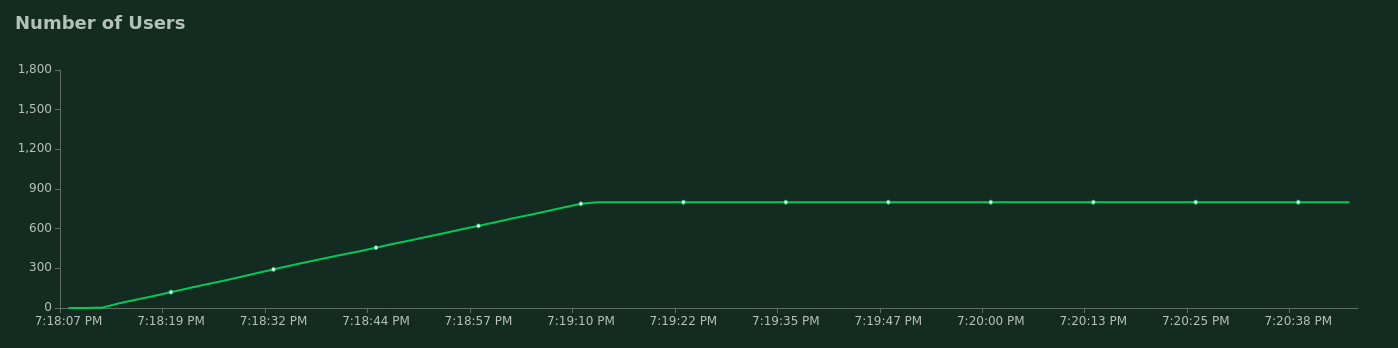
\includegraphics[width=\linewidth]{tests/local/800/number_of_users_1588097887.png}
%   \end{minipage}%
%   \label{fig:LocalTests:number_of_users}
%   \begin{minipage}{\textwidth}
%     \centering
%     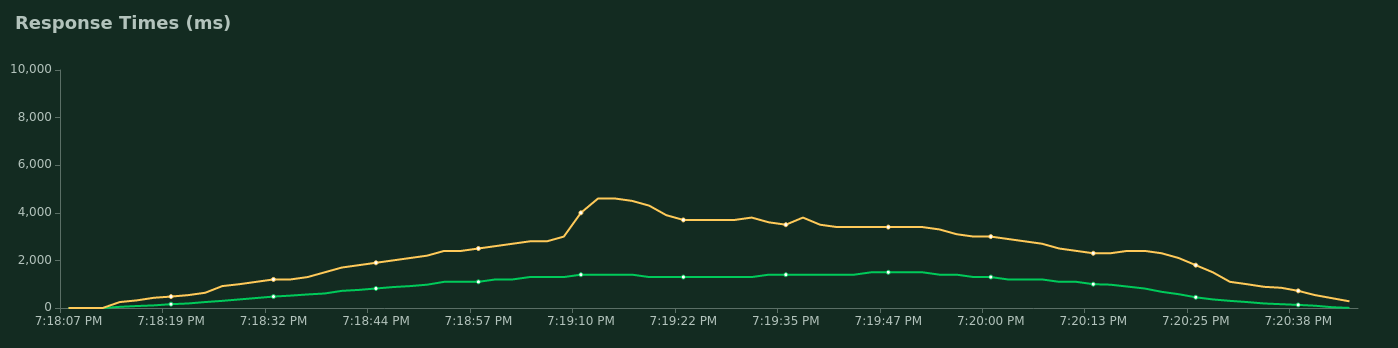
\includegraphics[width=\linewidth]{tests/local/800/response_times_(ms)_1588097887.png}
%   \end{minipage}%
%   \label{fig:LocalTests:response_times_(ms)}
%   \begin{minipage}{\textwidth}
%     \centering
%     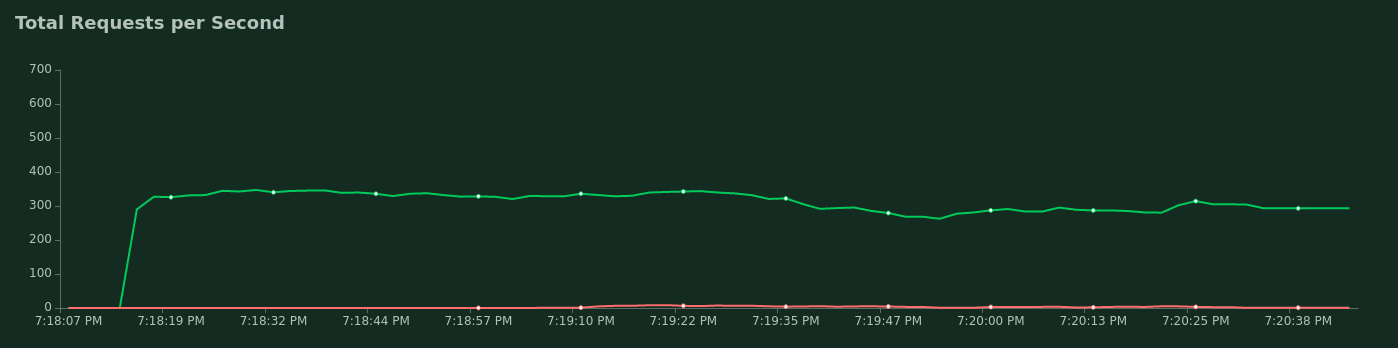
\includegraphics[width=\linewidth]{tests/local/800/total_requests_per_second_1588097887.png}
%   \end{minipage}%
%   \caption{Load tests results with 800 users.}
%   \label{fig:LocalTests:total_requests_per_second}
% \end{figure}
% \vspace{-10pt}

\newpage
\section{System Architecture} \label{architecture} %%%%%%%%%%%%%%%%%%%%%%%%%%%%%%%%%%%%%%%%%%%%%%%%%%%%%%%%%%%%%%%%%%%%%%%%%%%%%%%%%%%%%%%%%%%%%%%%%%%%%%%%%%%%%

\subsection{Infrastructure} \label{architecture.infrastructure} %%%%%%%%%%%%% 

% What is the architecture of the infrastructure deployed?

To provide the Pretix Ticketing Software to the public, it was required to set up an infrastructure containing their Django-based web application, an instance
of a Web Server Gateway Interface (WSGI) hosting the application and of a reverse-proxy for the web application deployment in production mode, as well as a
database management system (DBMS) (where PostgreSQL was used) for handling disk storage and a caching server (where Redis was chosen) for in-memory storage and
asynchronous queuing of tasks.

Our strategy is thoroughly described in the previous report, which already considered minimum redundancy to ensure availability.
It is achieved through the usage of Docker to isolate each component for greater control and easier configuration, and Docker Swarm for the orchestration of
the entire infrastructure.
Nevertheless, as it was a still primitive solution, naturally several upgrades were applied, mostly internally to each container.
The latest architecture is visually presented in Figure \ref{fig:InfrastructureArchitecture}.
This solution considers quality attributes whose assurance is described in the sections below.

\begin{figure}[H]
  \centering
  \begin{minipage}{.85\textwidth}
    \centering
    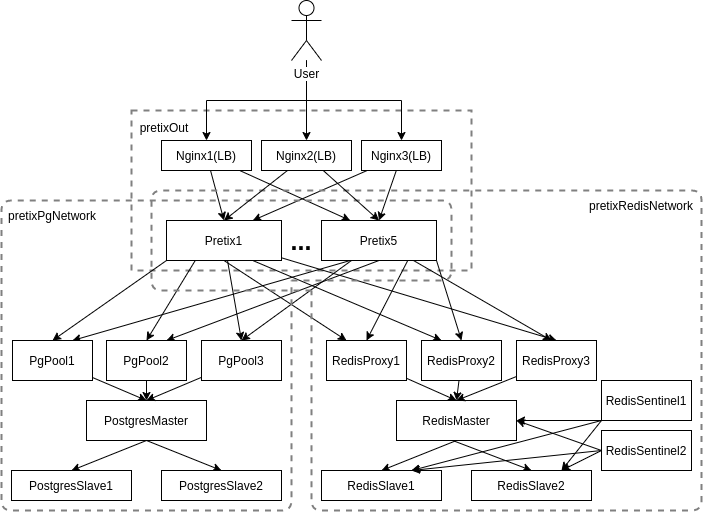
\includegraphics[width=\linewidth]{diagrams/InfrastructureArchitecture.png}
  \end{minipage}%
  \caption{Infrastructure architecture diagram deployed in Docker Swarm.}
  \label{fig:InfrastructureArchitecture}
\end{figure}

\subsection{Load Balancing} \label{architecture.loadbalancing} %%%%%%%%%%%%%

% How is load balancing assured?

The knowledge gathered so far regarding the operation of Pretix affirms that user activity peaks are to be expected when in production.
This has many implications and requires the implementation of mechanisms that maximize the infrastructure's efficiency.

With this in mind, we have come up with mechanisms for load balancing based on proxy servers.
These servers, when strategically placed, act as intermediaries for requests seeking resources from the system itself.
This not only reduces the complexity of requests made to our services, but also provides additional benefits with regards to security and load balancing,
as they allow a controlled and intelligent distribution of requests among components.

An NGinX proxy was installed between the end users and the web application.
With the help of Docker Swarm, replicas of both the proxy and the web application were deployed.
This is transparent for the user and it works as if he/she is sending requests to one single access point.

The storage clusters also resort to proxies.
For the PostgreSQL server cluster, we adopted Pgpool-II.
As our database is replicated in master/slave mode, Pgpool is able to take advantage of the replication feature in order to reduce the load on each PostgreSQL server
by evenly distributing queries among available servers and consequently improving the overall throughput.
Pgpool provides other useful features such as connection pooling, where it maintains established connections to the servers and reuses them whenever a new
connection with the same properties comes in, and automated fail over, mentioned in greater detail in section \ref{management.automation}.

For the Redis server cluster, the adopted solution was the well-known HAProxy.
The instances installed spread requests evenly across the Redis cluster.
Here, a master/slave mode was also used, meaning that the proxies interact with master instances that then delegate work among slaves.

Load tests executed during development proved that such additions had a significant impact on the performance of the system.
The usage of networks, seen in Figure \ref{fig:InfrastructureArchitecture}, where the proxies mentioned above are inserted help orchestrating and logically
grouping components.

\subsection{Redundancy} \label{architecture.redundancy} %%%%%%%%%%%%%%%%%%%%

% How is redundancy assured?

In order for us to provide Pretix, it is only required to maintain one instance of each component running.
However, this is highly unadvisable as it susceptible to failure from any point, i.e. if any of the system components fails, the entire system goes down.
This is referred to as a redundancy measure of N.

Ensuring actual redundancy of a system requires at least a measure of N+1, where each component can be replaced by another if required.
In most cases this is achievable through the replication feature of Docker Swarm.
Pretix's stack has K replicas of NGinX, of the Pretix web application, of Pgpool proxy and of HAProxy, where K can be defined on deployment with a value greater than 2.

Redundancy was also the reason why a master/slave mode was adopted on both clusters.
By instantiating 1 master and K slaves, it is possible to fulfill the requirements implicit to N+1 since if any slave fails the others can replace it and if the
master fails a slave is elected the new master.
Fortunately, for the PostgreSQL cluster this reelection process is done automatically, but for the Redis cluster the use of sentinels is required: sentinels
observe the behavior of masters and slaves, detect failures and reassign roles when needed; here we insist on providing N+1 redundancy by having multiple
instances of sentinels as well.

\subsection{Scalability} \label{architecture.scalability} %%%%%%%%%%%%%%%%%%%%%

% How is horizontal scalability assured?

Any project intended to be successful must consider the scalability of the product in the future.
Ours is no exception since, if the ticketing platform becomes popular, the infrastructure must be prepared to respond to greater loads of income traffic.

There were 2 means to ensure scalability: vertical or horizontal.
As we had access to limited computational resources and adding more physical RAM or CPUs was not an option, the only alternative left was to support horizontal scaling.

The idea here is to make possible the deployment of new replicas of any component and integrate them to the existing infrastructure without significant negative
impact on insertion and in a completely transparent way to the users.
This is exactly what we achieved.
Additionally, each component identifies itself to the monitoring server on initialization so that the data related to what is being managed is constantly up-to-date.

Scaling a portion of the stack can be done both manually or in an automated way.
By default we support manual scaling, but we found it was logical to implement automated mechanisms to scale up or down according to the online users and the
resources used.
This was achieved through the monitoring of meaningful metrics collected from each container instance, as we present in section \ref{management.automation}.

\newpage
\section{Infrastructure Management} \label{management} %%%%%%%%%%%%%%%%%%%%%%%%%%%%%%%%%%%%%%%%%%%%%%%%%%%%%%%%%%%%%%%%%%%%%%%%%%%%%%%%%%%%%%%%%%%%%%%%%%%%%%%%%

\subsection{Service Level Agreement} \label{management.sla} %%%%%%%%%%%%%%%

% What are the SLAs defined?

As service providers, we are supposed to fulfill a commitment with our clients, whether it is formally defined or not.
Obviously it is a good practice to elaborate an agreement where particular aspects of the service are agreed between the service provider and the service user -
this is called a Service Level Agreement (SLA).
We describe ours in this section.

Considering the scope of our project, we've defined the following commitment key points:
\vspace{-10pt}
\begin{itemize}[noitemsep]
  \item Pretix is to be provided through web browsers, by accessing a particular address, and it will only be accessible to those within the university's virtual private network (VPN).
  \item Its usage is fully dependent on the usability of the Pretix service itself and no complexity should be added by the infrastructure we provide with regards to this.
  \item We are responsible for providing free access to the ticketing platform through our servers and keeping data integrity even when the service is unavailable
  \item The installations hosting our deployment belong to a third party (the university) and thus we are not accountable for possible availability issues related to networking and machine up time.
        Nevertheless, if this is not considered, we ensure an availability of 100\% under normal circumstances and of 70\% for high activity peaks \footnote{Over 50 requests per minute.}, with a maximum response time of 50 seconds for ticket purchasing requests.
  \item No support is guaranteed for issues about features related to the internal implementation of the ticketing software.
\end{itemize}
\vspace{-10pt}

It is worth mentioning that our analysis to the (free version of the) Pretix product showed that the software had strong limitations on maximum load capacity
and response time that, according to the authors, could not be solved through horizontal scaling.

Focusing on the infrastructure itself and the computational resources, we have defined a list of Service Level Objects (SLO) - the metrics to be observed -
representative of the stack's state, and a list of Service Level Indications (SLI) - the thresholds or functions applied to the metric values - that will
help us react to situations where the SLA compliance is threatened.
These SLOs revolve around: hardware capacity, operation latency, availability percentage and reliability.

Table \ref{tab:sla} presents a simplified view on the metrics used to monitor the SLA and some thresholds that aid on the prevention of a cop-out.

\begin{table}[h!]
  \begin{center}
    \begin{tabular}{l|l|r}
      \hline
      \textbf{Category}   & \textbf{Metric}         & \textbf{Upper Threshold}  \\
      \hline 
      Hardware            & System Up Time          & -                         \\
      (SNMP)              & \% User CPU Time        & 90\%                      \\
                          & Total RAM               & -                         \\
                          & Total RAM Used          & -                         \\
                          & \% RAM Usage            & 90\%                      \\
                          & Total Disk              & -                         \\
                          & Total Disk Used         & -                         \\
                          & \% Disk Usage           & 90\%                      \\
      \hline
      Pretix              & Total \# of Events      & -                         \\
                          & Total \# of Orders      & -                         \\
                          & Total \# of Purchases   & -                         \\
                          & Response Time           & 50 seconds                \\
      \hline
      NGinX               & Total \# of Requests    & 10\% (failure)            \\
                          & Average Response Time   & 50 seconds                \\
      \hline
      Redis               & Redis Up Time           & -                         \\
                          & Memory Used             & -                         \\
                          & \# of Connections       & -                         \\
                          & \# of Connected clients & -                         \\
      \hline
    \end{tabular}
    \caption{Monitored metrics, categorized by source.}
    \label{tab:sla}
  \end{center}
\end{table}

\subsection{Monitoring} \label{management.monitoring} %%%%%%%%%%%%%%%%%%%%%

% How is the infrastructure monitored? 
% SNMP, logs, metrics exporters

Understanding the state of the infrastructure and components is essential for ensuring the correct functioning and stability of the service.
Information about the health and performance of deployments not only helps us react to issues, it also gives security to make changes with confidence. 
One of the best ways to gain this insight is with a robust monitoring system that gathers logs and metrics, visually displays data, and alerts us operators when 
undesired events occur or when the maximum capacity of some resource is almost reached.
This kind of system also allows the definition of reactions for specific SLA violation threats.

Our monitoring system is hosted on an independent machine with 32 cores of 2.1GHz, 64Gb of RAM and 7Tb of disk space.
Just as the infrastructure hosting our Pretix stack, this too was shared amongst other operator teams.
The virtual machine (VM) we instantiated for our monitoring system runs Ubuntu 20.04 LTS and has 2 CPU cores, 4Gb of RAM and 50Gb of disk space.
The separation between our product and its monitoring was understood to be optimal, since this way there is no added load to the service facility, keeping its
resources fully dedicated to itself.
There is also the advantage of allowing the deployment of our system both with or without monitoring enabled.

\subsubsection{Log Collection}
Log collection, as the name implies, consists in gathering in a centralized fashion all the logs generated by all services composing our full system. There are a lot of options to achieve this, some that we considered and investigated. To analyze the logs themselves in a user-friendly and feature rich platform we choose the Elasticsearch stack(ELK), comprised of Elasticsearch itself, Logstash and Kibana. The purpose of each of those components are:

\begin{itemize}
  \item Elasticsearch - text based database, optimized to search and filter through textual data,, such as logs.
  \item Logstash - textual data(logs) collector/receiver; stack entrypoint.
  \item Kibana - GUI data analyzer, enabling the creation of dashboards, alerts, ...
\end{itemize}

One of the approaches we tested the centralize all logs but ended up not being used in the final product was the rsyslog approach. This technology allows the definition of a server and multiple clients, each one assigned to each service, that gathers the system logs of the machine and sends them to the predefined rsyslog server. Although enabling a centralized registry of all logs of the system's services, some integration problems were encountered but after some analysis we found this option not to be optimal, since the rsyslog when receiving exterior logs will persist them in the system logs file of the hosting machine. Since this entity would be hosted by the monitoring virtual machine, every log received would be replicated since the rsyslog persists them and the Elasticsearch would also persist them due to it's indexing process.

The approach we settle on ended up being much cleaner and simpler in our opinion. After some research we found that one of the logging drivers provided by the docker platform was syslog, that enables the redirecting of all logs to a syslog server specified in the driver options. This was exactly aligned with our scenario, since all our deployment was made in docker's swarm mode and we wanted to centralize all services logs. We also found that Logstash allows the creation of a server that can receive any type of message(since filters can be applied to the incoming messages), enabling the direct connection between the docker syslog driver and the ELK stack.

After the logs arrive at the Logstash, the internal ELK flow was configured so that Elasticsearch indexes the information and Kibana is able to access it. The system is then capable of collecting all logs and present them in the Kibana interface, enabling a centralizes analysis and further alert definition.

Further processing over collected logs can be made if the information is context specific and allows these type of processing, such as counters or other metrics. In our case we concluded that this was not necessary since we were able to obtain metrics from all the services necessary, information we processed with the technologies described in the following subsection.

\subsubsection{Metric Collection}
Metric collection is very similar to log collection in the sense that the objective is to centralize all generated information from all the system's composing services, but this time the data collected are metrics, most of the time numeric data like counters, gauges and indicators about the service process itself or even context specific ones.

Obviously, there are many approaches and technologies that allow metric collection. After some investigation we found some that are commonly used for this purpose, such as Nagios, Zabbix, Munin, TICK stack, Prometheus and more. We opted to implement the Prometheus one, since our main service(Pretix) already exported metrics in the Prometheus format. For the remaining services we needed to install parallel metric exporters compatible with Prometheus. Since our infrastructure was deployed using docker in swarm mode, the addition of exporters was made by changing the Dockerfiles and respective entrypoints for each service. The mapping between service and installed exporter was:

\begin{itemize}
  \item Nginx - 
  \item Pg Master/Slave - 
  \item HA Proxy - 
  \item Redis Master/Slave/Sentinel - 
\end{itemize}

In addition to all those exporters, we also installed another one in the monitoring virtual machine itself responsible for monitoring the hardware itself, like the CPU, memory and disk usage. For that task we used the SNMP protocol, which is a internet standard protocol for collecting and organizing information about managed devices on IP networks and for modifying that information to change device behavior. The protocol support was installed a priori on every compute node, being only necessary request it's metrics when necessary. Since the deployment is made using the Docker's Swarm mode, it was impossible for us to know were our services would be deployed in the Swarm computing network. With that in mind we had two options: either we statically indicated every computing node to be monitored, or we dynamically discovered the ips of the machine hosting our services. We concluded that the first option was not feasible since it would cause unnecessary stress in machines and would not scale well, since if there were 1000 computational nodes we would need to indicate the 1000 ips. We opted to dynamically discover the machine ips, which implied that we needed to create a custom ip collector.

This custom component had an independent service and was created using Python's Flask library, which enabled us to quickly develop the necessary endpoints and respective logic. At initialization, each service sends a HTTP Post to our custom service with its name, replication number and id. Our service will then register or update it's ip and modify the respective Prometheus target files for each type of exporter.

Prometheus is the engine behind the monitoring and alerting, but it's as necessary a powerful, usable and efficient user interface. Grafana is commonly integrated with Prometheus, being the GUI indicated by the engine itself. That was the reason we deployed Grafana, enabling us to explore the collected metrics, construct meaningful dashboards and configuring critical alerts.

\subsection{Alerts and Automation} \label{management.automation} %%%%%%%%%%%%%%%%%%%%%

% SLA violation alarms
% How is the provisioning of new elements automated?
% How is the infrastructure fault tolerant? (pgpool automated failover, redis sentinels, SLA violation alarm responses)
Collecting metrics and logs means nothing if there's no objective. For that reason we defined the SLA described in section \ref{management.sla}, enabling us to know when the infrastructure and system are performing as expected or not. When the SLA is violated the system should notify the infrastructure manager so that a action may be performed. In more advanced scenarios, automatic reactions may be specified so that the system can adjust to certain problems, creating some desirable flexibility.

For our context and service, we defined both alerts and automatic responses. Alerts were configured in every metric considered critical and that it's behavior may translate in the status of the service, as explained in section \ref{management.sla}. All the generated alarms and notifications were made by a Microsoft Teams channel. All those alarms were also sent to a custom service responsible for receiving, processing and if necessary reactive to the incoming alarms. This service was the same as the one responsible for collecting the computing machines for efficiency reasons. When receiving an alarm, the component will process it and if it's one that can be corrected in an automatic fashion, a reaction will be executed, in our case, using the Docker's Python SDK to automatically scale up or down the service that triggered the alarm. The alarms and respective reaction are:

\begin{itemize}
  \item
\end{itemize}

\newpage
\section{Additional Remarks} \label{remarks} %%%%%%%%%%%%%%%%%%%%%%%%%%%%%%%%%%%%%%%%%%%%%%%%%%%%%%%%%%%%%%%%%%%%%%%%%%%%%%%%%%%%%%%%%%%%%%%%%%%%%%%%%%%%%%%%%%%

\subsection{Swarm Stability} \label{remarks.stability} %%%%%%%%%%%%%%%%%

% issues with pgpool

...

\subsection{Assignment Contributions} \label{remarks.contributions} %%%%%%%%%

% who did what?

Due to external issues that prevented physical proximity among students and professors, a confined approach had to be adopted during this second development phase.
Nevertheless, the close-contact strategy was kept as this project required a broad perspective on the infrastructure and the tasks to be implemented by both team members.
Regarding the work distribution among developers, tasks were assigned to each according to a predefined plan and a common working schedule was applied. 

The technology-related decisions were first made in conjunction.
Then, Filipe set up the monitoring VM to gather the data from the stack while João began to work on the mechanism to collect the logs from each container.
Filipe moved on to installing metric exporters on each container, and João found means to collect lower level metrics using the SNMP.
The container identification mechanism of each instance to the monitoring system was then implemented.
At this stage, both operators worked on defining the SLA and João designed the monitoring dashboards.
Finally, the alarms and automated response mechanisms were implemented.
It is needless to say that bug and error solving was made along the development phase by both developers any time it was required.
Once a stable deployment fulfilling all predefined requirements was completed, this report became our primary concern, with both contributing equally.

\newpage
\section*{Conclusions} \label{conclusions} %%%%%%%%%%%%%%%%%%%%%%%%%%%%%%%%%%%%%%%%%%%%%%%%%%%%%%%%%%%%%%%%%%%%%%%%%%%%%%%%%%%%%%%%%%%%%%%%%%%%%%%%%%%%%%%%%%%%%

...

\newpage
\begin{thebibliography}{9} %%%%%%%%%%%%%%%%%%%%%%%%%%%%%%%%%%%%%%%%%%%%%%%%%%%%%%%%%%%%%%%%%%%%%%%%%%%%%%%%%%%%%%%%%%%%%%%%%%%%%%%%%%%%%%%%%%%%%%%%%%%%%%%%%%%%%
  \bibliographystyle{Science}

  \bibitem{assign}
  J. P. Barraca,
  \textit{GIC - Report no.2: Simple Product Operation},
  University of Aveiro,
  2019/20.
  \vspace{-10pt}

  \bibitem{pretix}
  \textit{About Pretix},
  \url{https://pretix.eu/about/en/}.
  Pretix.eu,
  retrieved in April 2020.
  \vspace{-10pt}

  \bibitem{rami.io}
  \textit{Welcome to Rami.io},
  \url{https://rami.io/}.
  Rami.io,
  retrieved in April 2020.
  \vspace{-10pt}

  \bibitem{pretixgit}
  \textit{Pretix Code Repository},
  \url{https://github.com/pretix/pretix}.
  GitHub, Inc.,
  retrieved in April 2020.
  \vspace{-10pt}

  \bibitem{pretixdoc}
  \textit{Welcome to pretix' documentation!},
  \url{https://docs.pretix.eu/en/latest/}.
  Pretix.eu,
  retrieved in April 2020.
  \vspace{-10pt}

  \bibitem{docker}
  \textit{Docker Homepage},
  \url{https://www.docker.com/}.
  Docker Inc.,
  retrieved in April 2020.
  \vspace{-26pt}

  \bibitem{pretix_img}
  \textit{pretix/standalone},
  \url{https://hub.docker.com/r/pretix/standalone}.
  pretix,
  retrieved in April 2020.
  \vspace{-10pt}

  \bibitem{django}
  \textit{Meet Django},
  \url{https://www.djangoproject.com/}.
  Django Software Foundation and individual contributors,
  retrieved in April 2020.
  \vspace{-10pt}

  \bibitem{gunicorn}
  \textit{Gunicorn Homepage},
  \url{https://gunicorn.org/}.
  Gunicorn.org,
  retrieved in April 2020.
  \vspace{-10pt}

  \bibitem{nginx}
  \textit{NGinX News},
  \url{https://nginx.org/}.
  NGinX.org,
  retrieved in April 2020.
  \vspace{-10pt}

  \bibitem{postgresql}
  \textit{PostgreSQL: The World's Most Advanced Open Source Relational Database},
  \url{https://www.postgresql.org/}.
  The PostgreSQL Global Development Group,
  retrieved in April 2020.
  \vspace{-10pt}

  \bibitem{redis}
  \textit{About Redis},
  \url{https://redis.io/}.
  Redis Labs,
  retrieved in April 2020.
  \vspace{-10pt}

  \bibitem{pgpool}
  \textit{Welcome to Pgpool-II},
  \url{https://www.pgpool.net/mediawiki/index.php/Main_Page}.
  PgPool Global Development Group,
  retrieved in April 2020.
  \vspace{-10pt}

  \bibitem{haproxy}
  \textit{HAProxy: The Reliable, High Performance TCP/HTTP Load Balancer},
  \url{https://www.haproxy.org/}.
  HAProxy.org,
  retrieved in April 2020.
  \vspace{-10pt}

  \bibitem{locust}
  \textit{Locust, an open source load testing tool},
  \url{https://locust.io/}.
  Locust.io,
  retrieved in April 2020.
  \vspace{-10pt}

  \bibitem{selenium}
  \textit{About Selenium},
  \url{https://www.selenium.dev/about/}.
  Software Freedom Conservancy,
  retrieved in April 2020.
  \vspace{-10pt}

  \bibitem{ansible}
  \textit{Ansible},
  \url{https://www.ansible.com/}.
  Red Hat,
  retrieved in April 2020.

\end{thebibliography}

\clearpage

\end{document}




















